\documentclass{article}
\usepackage[utf8]{inputenc}
\usepackage{enumitem}
\usepackage{graphicx}
\usepackage{color}
\usepackage{rotating}
\usepackage{adjustbox}

\title{Next Generation User Interface: \\Redefining file browsing}
\author{
  De Bleser, Jonas\\
  \texttt{jdeblese@vub.ac.be}\\
  Rollnumber: 0508848
  \and
  Carraggi, Nicolas\\
  \texttt{ncarragg@vub.ac.be}\\
  Rollnumber: 0093262
  \and
  Spruyt, Valentijn\\
  \texttt{vspruyt@vub.ac.be}\\
  Rollnumber: 0508466
}
\date{\today}

\begin{document}

\maketitle


\tableofcontents

\section{Problem statement}
The current state of file browsing is very similar on most desktop platforms. Based on an observation of the current file browsers, we conclude that each file browser consists of two important parts: a tree view and a content view. The first view shows the hierarchy and structure of the file system, whereas the second view simply shows the contents of one level in the hierarchy.  We also note that browsing through these views is solely based on mouse and keyboard input. These observations exists for quite a long time and have not changed in the past decades. Therefore, our goal is to redefine file browsing by means of hand gestures, a flat file hierarchy and a more simple, intuitive interface. In the end, we are not really trying to solve a problem, but we rather want to create another approach towards file browsing.

Our approach consists of groups and tags to create a flat, nevertheless usable, hierarchy of files. A group is a general representation of a cluster of files. A tag is similar to a label and represents a keyword (e.g. vacation, Belgium, cat). A group is created by assigning it a name and several tags. Those tags determine which files will be related to this group. Assuming we add the tags \texttt{vacation} and \texttt{Belgium} to a group, it will cluster all files that have one of the aforementioned tags into that group. We decided to not support the feature of nested groups, because we want a clear overview of all groups. Nevertheless, nesting can also be achieved using our system. For example.. TODO. In terms of customizability, groups and tags can also have a color to characterize the appearance.

\section{Requirements analysis}

\subsection{Usability requirements}

\begin{enumerate}
\item 
    \begin{itemize}[label=$ $]
    \item \textbf{Description:} Checking the events per day should be possible within 2 steps starting from the main view
    \item \textbf{Motivation:} Since this is one of the principal aims of the system, it may not be difficult to do this. The user should be able to go to the next, previous or calendar day in one step, as well as applying a filter using another step.
    \item \textbf{User class(es):} User
    \item \textbf{Measuring concept:} User satisfaction
    \item \textbf{Measuring method:} Task scenario
        \begin{itemize}
        \item \textit{Result:} Amount of steps to perform the task
        \end{itemize}
    \item \textbf{Criteria for judging:}
        \begin{itemize}
        \item \textit{Worst level:} 3 or more steps
        \item \textit{Planned level:} 2 steps - using the calendar as well as the filter
        \item \textit{Best level:} 0 steps - The best possible level is zero because checking the events of the current day requires no additional steps
        \end{itemize}
    \end{itemize}
\end{enumerate}
    


\section{Design and iteractions}
 Nicolas Omer zei:

"interaction" was describing how the potential user would interact with the application. In our case, it is an Android application on a smartphone so it is via the touch screen, simple gesture, he uses tabs to navigate, push buttons, etc... (we explain all the things that have to be known to access every feature of the application)

So in our case that would be the 5 movements you have for the Myo I imagine + the fact that you can use another screen than the one of your computer, etc...

For the "design", we did pretty much the same than in the section "Style guidelines" for the project of the "User Interface Design" course (don't know if you have this one). 

Anyway : we describe how the design process was conducted (how we  came to such layout / display). Why a list view is better for storing your accounts (since you could have many), that we have drop-down menus to select a specific item in a list, etc... 

Don't know if that is what they expect but it's what we have wink-emoticon

\section{Technical report}

Inleidend tekstje

\subsection{Architecture}

We based our architecture on Java to support multiple platforms. We have tested our application on both Windows and Mac to make sure our application works correctly. Metadata for our application is stored using HSQLDB\footnote{http://hsqldb.org} (HyperSQL DataBase). We also use Node.js\footnote{https://nodejs.org} as a web server to serve files to the front-end.  The user interface is build using HTML, CSS and JavaScript frameworks such as Bootstrap\footnote{http://getbootstrap.com}, Backbone.js\footnote{http://backbonejs.org}, Marionette.js\footnote{http://marionettejs.com} and Require.js\footnote{http://requirejs.org}. We made the decision to make the graphical user interface web-based, since it is a lot easier to customize the look and feel, as well as do advanced animations. To display the web content, we use JXBrowser which is a Java-based browser supporting Webkit\footnote{https://webkit.org}. Backbone.js is an MV* framework which provides us models, collections, views and additional functionalities to glue them together. However, it is very low level framework and therefore we use Marionette.js on top of it which gives us higher level components. For example, a \texttt{CollectionView} which provides us with all logic and functionalities to display a collection. In Backbone.js we would have to create such a common-used view from zero. We also use Require.js to work with dependencies for each file. In this way, only the required dependencies are fetched from the server, limiting the amount of requests to the server. However, once the application is finished, we can minify all dependencies to one file and simply load it using JXBrowser. As a result, we could remove the Node.js based web server entirely, but we left it for development purposes. Specifically, the only reason Node.js is used, is to avoid the same-origin policy problem with local dependencies. We also used a Java port\footnote{https://github.com/NicholasAStuart/myo-java} of the Myo SDK, instead of the default C/C++ SDK.

\subsection{Challenges}

In this section we will discuss some of the challenges we encountered during the development of our project.

\subsubsection{The Marionette.js framework}
One of the biggest challenges of this project was the Marionette.js\footnote{http://marionettejs.com} framework itself. Even though only one member of our team had experience with the framework, we all agreed on using it. The motivation for using this framework was that it has a neatly built model and view structure, which made it possible to write clean code that is fairly easy to read. The framework itself is a decent framework, but development went very slow because of the basic knowledge of JavaScript by the other two members. On the other side: Using this framework really upped our JavaScript skills, which will be handy for the future.

TODO: Jonas zet nog wa bij die motivatie as ge wilt over marionette. 

\subsubsection{Myo}
The Myo\footnote{https://www.myo.com/} bracelet is a something which can be used in a wide range of applications. When we watched a demo video, we immediately thought that it would be a nice thing to use for uit NGUI project. The nice thing about the bracelet is that it already supports several basic gestures and that it can detect spatial arm movement, next to just gestures of the lower-arm. However, when we started the project, we thought of adding custom gestures which were detectable by the bracelet. We saw fairly soon that this wouldn't be optimal since it was already difficult enough for the bracelet to detect the basic gestures. This was a big issue for the development of our project. When we tried to test our application with gesture \texttt{X}, the chances were that the bracelet detected gesture \texttt{Y} instead, which lead to great frustration.
Another issue was the problem that comes with working with hardware, rather than software alone: Only one team member could take the Myo bracelet home and do some testing and programming with it. This caused delays in the development process, since it was very hard to synchronize work progress. An example: We decided to implement feature \texttt{A} in our application. One teammember had set up the layout and views of the feature, another member coded some processing functions for the feature and the third teammember was in charge of writing the code to send the myo gestures to our clientside JavaScript. The problem was that, obviously, not everyone could work for the project 24/24 hours every day. This made development slower because we sometimes had to wait on another member to finish his assigned task. The other members couldn't just go and drive several tens of kilometers to go and fetch the Myo bracelet, so that they could write the code themselves.
A last issue was that the Myo bracelet needs some warming up and synchronization before you can use it. This synchronization phase requires the user to perform a \textit{wave-out} gesture for several seconds to even a minute long. This resulted into cramps in our lower arm more than once.

TODO: NICO iets over calibratie ofzo?


\subsubsection{JxBrowser}
Tijd om license te krijgen
responsiveness enzo, events doorsturen,

To bridge the gap between Java and JavaScript, we used the JxBrowser component. When we initially looked the component up, it looked very promising. A 30-day trial was available so we could start right away. After that we could get a free educational license, after filling in some forms. We soon realized that the JxBrowser component was rather processor-heavy, and that its responsivenes was sometimes rather low. The component came in the form of a \textit{.jar} file, and modified something in the registry of our computer, so that we couldn't just use a new 30-day trial when the old one expired. This lead to several problems. In order to obtain an educational license, we first had to fill in a form with some information about the VUB. After that, we also had to ask Dr. Signer to send a recommandation mail to confirm that we are indeed students at the VUB. When the developers of the JxBrowser component finally sent us the license, it didn't work. There was some sort of bug that didn't change the registry key, so we kept getting the error that our 30-day trial had expired. By the time that we figured this out together with the developers, we had lost quite some time.

Todo jonas over JS single threaded shit

\newpage
\section{Evaluation}

\subsection{Self-evaluation}
TODO ALOT OF TEXT

\subsection{Evaluation by others}
In this section we will discuss how others evaluated our project. First, we will take a look at the results from te questionnaire. After that, we will discuss these results by analyzing the feedback that we got from the evaluators.
\newpage
\subsubsection{Questionnaire}

\begin{itemize}
		\item[] \textbf{Question 1:} I think I would use the product often
		\item[] \begin{minipage}[t]{\linewidth}
         	 \raggedright
          	\adjustbox{valign=t}{%
            		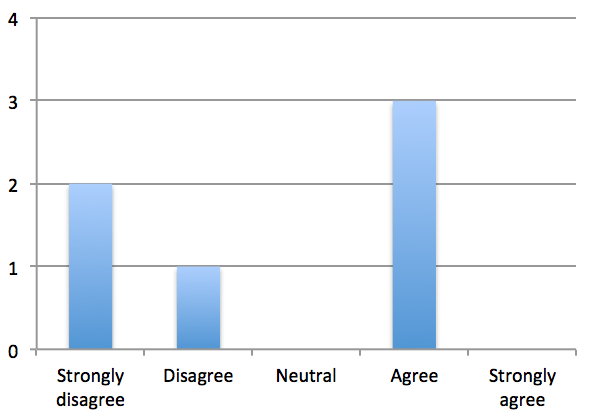
\includegraphics[width=1\linewidth]{./Images/graph1.png}%
          	}
          	\medskip
          	\centerline{Graph 1: Answers to question 1}
          \end{minipage}
\end{itemize}
\begin{itemize}
		\item[] \textbf{Question 2:} I find the product unnecessarily complex
		\item[] \begin{minipage}[t]{\linewidth}
         	 \raggedright
          	\adjustbox{valign=t}{%
            		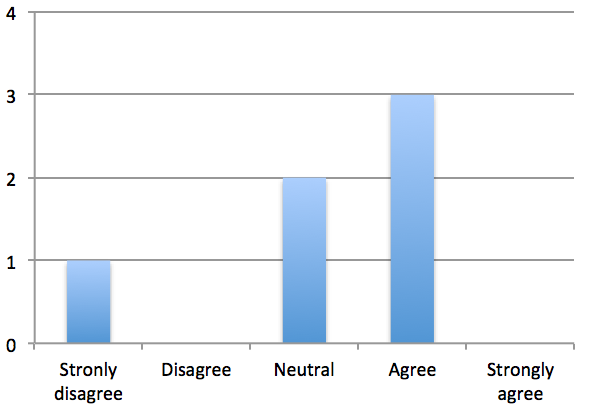
\includegraphics[width=1\linewidth]{./Images/graph2.png}%
          	}
          	\medskip
          	\centerline{Graph 2: Answers to question 2}
          \end{minipage}
\end{itemize}
\begin{itemize}
		\item[] \textbf{Question 3:} I find the product easy to use
		\item[] \begin{minipage}[t]{\linewidth}
         	 \raggedright
          	\adjustbox{valign=t}{%
            		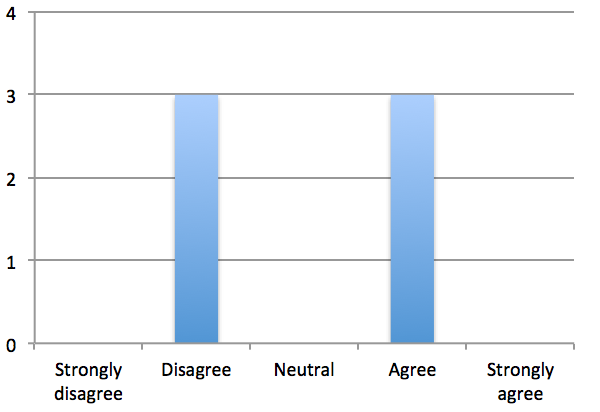
\includegraphics[width=1\linewidth]{./Images/graph3.png}%
          	}
          	\medskip
          	\centerline{Graph 3: Answers to question 3}
          \end{minipage}
\end{itemize}
\begin{itemize}
		\item[] \textbf{Question 4:} I think I would need a technical person to use this product
		\item[] \begin{minipage}[t]{\linewidth}
         	 \raggedright
          	\adjustbox{valign=t}{%
            		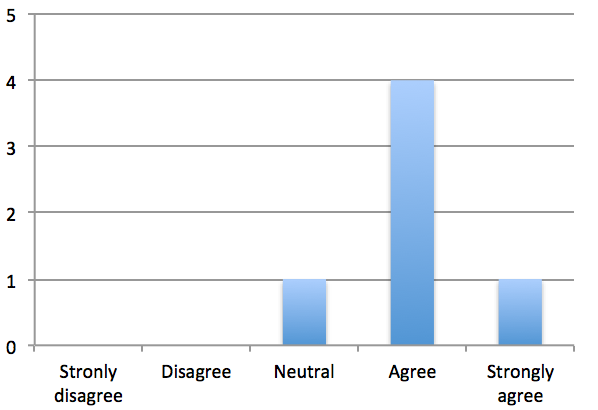
\includegraphics[width=1\linewidth]{./Images/graph4.png}%
          	}
          	\medskip
          	\centerline{Graph 4: Answers to question 4}
          \end{minipage}
\end{itemize}
\newpage
\begin{itemize}
		\item[] \textbf{Question 5:} I find that the different functions of the product are clear
		\item[] \begin{minipage}[t]{\linewidth}
         	 \raggedright
          	\adjustbox{valign=t}{%
            		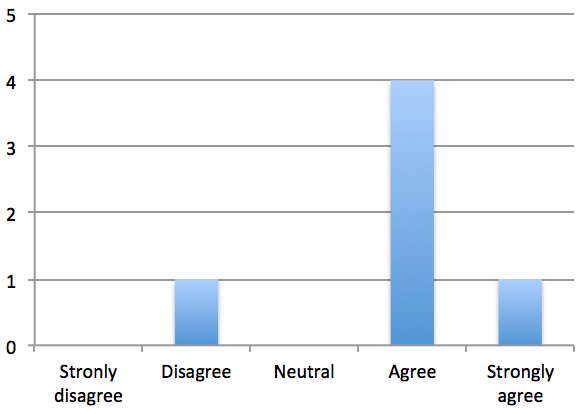
\includegraphics[width=1\linewidth]{./Images/graph5.png}%
          	}
          	\medskip
          	\centerline{Graph 5: Answers to question 5}
          \end{minipage}
\end{itemize}
\begin{itemize}
		\item[] \textbf{Question 6:} I find the product inconsistent
		\item[] \begin{minipage}[t]{\linewidth}
         	 \raggedright
          	\adjustbox{valign=t}{%
            		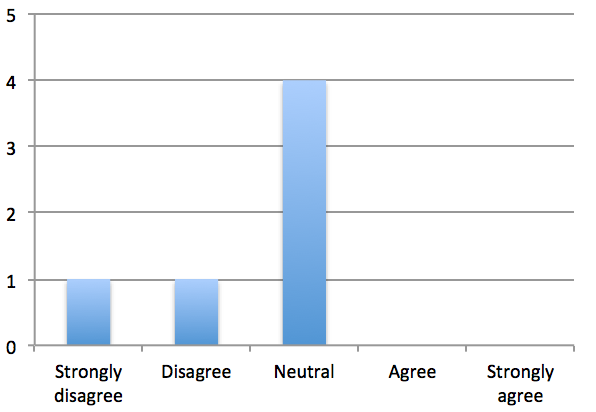
\includegraphics[width=1\linewidth]{./Images/graph6.png}%
          	}
          	\medskip
          	\centerline{Graph 6: Answers to question 6}
          \end{minipage}
\end{itemize}
\newpage
\begin{itemize}
		\item[] \textbf{Question 7:} I think most people will easily learn to work with the product
		\item[] \begin{minipage}[t]{\linewidth}
         	 \raggedright
          	\adjustbox{valign=t}{%
            		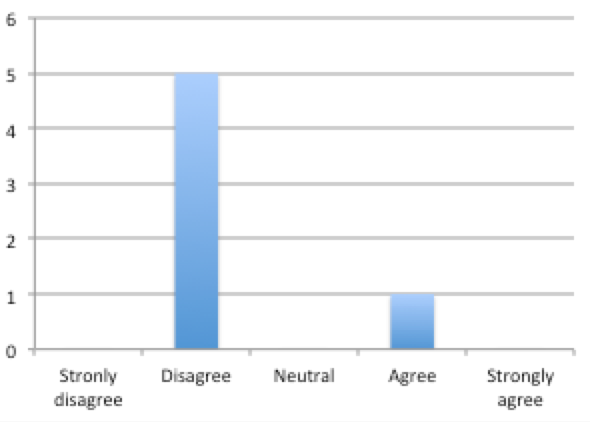
\includegraphics[width=1\linewidth]{./Images/graph7.png}%
          	}
          	\medskip
          	\centerline{Graph 7: Answers to question 7}
          \end{minipage}
\end{itemize}
\begin{itemize}
		\item[] \textbf{Question 8:} I find the product awkward to work with
		\item[] \begin{minipage}[t]{\linewidth}
         	 \raggedright
          	\adjustbox{valign=t}{%
            		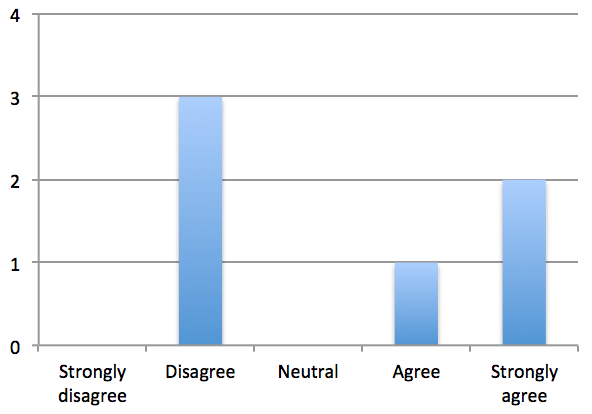
\includegraphics[width=1\linewidth]{./Images/graph8.png}%
          	}
          	\medskip
          	\centerline{Graph 8: Answers to question 8}
          \end{minipage}
\end{itemize}
\newpage
\begin{itemize}
		\item[] \textbf{Question 9:} I find it easy to see what functions are available when using the product
		\item[] \begin{minipage}[t]{\linewidth}
         	 \raggedright
          	\adjustbox{valign=t}{%
            		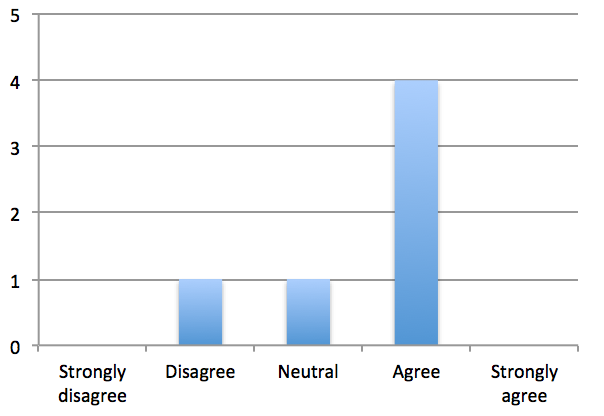
\includegraphics[width=1\linewidth]{./Images/graph9.png}%
          	}
          	\medskip
          	\centerline{Graph 9: Answers to question 9}
          \end{minipage}
\end{itemize}
\begin{itemize}
		\item[] \textbf{Question 10:} I had to learn a lot before being able to use the product
		\item[] \begin{minipage}[t]{\linewidth}
         	 \raggedright
          	\adjustbox{valign=t}{%
            		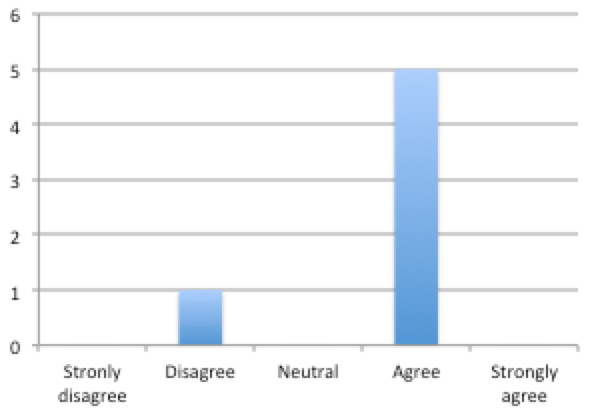
\includegraphics[width=1\linewidth]{./Images/graph10.png}%
          	}
          	\medskip
          	\centerline{Graph 10: Answers to question 10}
          \end{minipage}
\end{itemize}


\subsubsection{Explanation}











Source code (December 23): The source code of your next generation user interface together with
detailed and complete instructions on how to run it (i.e. step by step instructions together with possible
dependencies, required software and technologies, etc.). Note that your source code should be
documented: every important method and class should be annotated with a description of its goal and
functionality. If you use a tutorial, open source framework or other online code, you have to mention
this and cite the author’s website. We check for code plagiarism! The source code has to be sent to
Sandra Trullemans (strullem@vub.ac.be).

\end{document}
